\documentclass[a4paper, 12pt, twoside]{article}
\usepackage[T2A,T1]{fontenc}
\usepackage[utf8]{inputenc}
\usepackage[english, russian]{babel}
\usepackage{graphicx}
\usepackage[hcentering, bindingoffset = 10mm, right = 15 mm, left = 15 mm, top=20mm, bottom = 20 mm]{geometry}
\usepackage{multirow}
\usepackage{ gensymb }
\usepackage{lipsum}
\usepackage{amsmath, amstext}
\usepackage{siunitx}
\usepackage{subcaption}
\usepackage{wrapfig}
\usepackage{adjustbox}
\usepackage{enumerate, indentfirst, float}
\usepackage{capt-of, svg}
\usepackage{ctable}

\newcommand*{\hm}[1]{#1\nobreak\discretionary{} 
	{\hbox{$\mathsurround=0pt #1$}}{}}
\usepackage{cmap} % Улучшенный поиск русских слов в полученном pdf-файле

\usepackage{pscyr} % Нормальные шрифты
\usepackage[normalem]{ulem} % для подчёркиваний uline
\ULdepth = 0.16em

\usepackage{fancyhdr} %Колонтикулы
\pagestyle{fancy}
\lhead{
\includegraphics[width = 10 mm]{logo.jpg} Лабораторная работа № 4.3.3}
\rhead{\textit{17 февраля 2018 г.}}

\newenvironment{bottompar}{\par\vspace*{\fill}}{\clearpage}

\begin{document}
	\begin{titlepage}
		
		\newcommand{\HRule}{\rule{\linewidth}{0.7mm}} % Defines a new command for the horizontal lines, change thickness here
		
		\center % Center everything on the page
		
		%----------------------------------------------------------------------------------------
		%	HEADING SECTIONS
		%----------------------------------------------------------------------------------------
		
		\textsc{\LARGE Московский Физико-Технический Институт}\\[1,5cm] % Name of your university/college
		\textsc{\Large Кафедра общей физики}\\[0.5cm] % Major heading such as course name
		\textsc{\large Лабораторная работа \textnumero  4.3.3}\\[0.5cm] % Minor heading such as course title
		
		%----------------------------------------------------------------------------------------
		%	TITLE SECTION
		%----------------------------------------------------------------------------------------
		
		\HRule
		\\[0.4cm]
		{ \huge \bfseries Исследование разрешающей способности микроскопа методом Аббе}
		\\[0.2cm] % Title of your document
		\HRule
		\\[1.5cm]
		
		
		
		%----------------------------------------------------------------------------------------
		%	AUTHOR SECTION
		%----------------------------------------------------------------------------------------
		
		\begin{minipage}{0.4\textwidth}
			\begin{flushleft} \large
				\textbf{Автор:}\\
				Глеб Уваркин \\
				615 группа
			\end{flushleft}
		\end{minipage}
		~
		\begin{minipage}{0.4\textwidth}
			\begin{flushright} \large
				\textbf {Преподаватель:} \\
				Клёнов Сергей Львович % Supervisor's Name
			\end{flushright}
		\end{minipage}
		
		\begin{bottompar}
			\begin{center}
				
\includegraphics[width = 80 mm]{logo.jpg}
			\end{center}
			{\large \today}
			
		\end{bottompar}
		\vfill % Fill the rest of the page with whitespace
		
	\end{titlepage}
	
	{\Large \uline { \textbf  {Цель работы:}}}
	
	\vspace{2mm}
	Определение дифракционного предела разрешения объектива микроскопа методом Аббе.
	\vspace{\baselineskip}
	
	{\Large \uline { \textbf  {В работе используются:}}}
	
	\vspace{2mm}
	
	Лазер; кассета с набором сеток разного периода; линзы; щель с микрометрическим винтом; оптический стол с набором рейтеров и крепёжных винтов; экран; линейка.
	
	\section{Используемые формулы.}
	Для определения периода решёток имеем формулы :
	\begin{equation}
	\label{f1}
	d \sin \theta_x = m_x \lambda,~~~~~ d \sin \theta_y = m_y \lambda,
	\end{equation}
	
	где $m_x$ и $m_y$ -- целые числа, характеризующие порядки дифракционных максимумов, $\theta_x$ и $\theta_y$ -- направления на главные дифракционные максимумы в горизонтальной и вертикальной плоскостях соответственно.
	
	~
	
	Минимальное разрешаемое объективом расстояние определяется условием 
	
	\begin{equation}
	\label{f2}
	l_\text{min} \approx \dfrac{\lambda}{\sin A} \approx \dfrac{\lambda}{D/2f},
	\end{equation}
	
	где $D$ -- диаметр диафрагмы.
	
	~
	
	Увеличение системы линз рассчитывается по формуле (см. рис. \ref{scheme})
	$$ \Gamma = \dfrac{b_1b_2}{a_1a_2}$$\\
	
	
	

	\newpage
	\section{Экспериментальная установка.}
	Схема образования изображения в объективе микроскопа представлена на рис. \ref{img}. Для простоты рассмотрим случай, когда предметом является периодическая структура (дифракционная решётка), освещаемая параллельным пучком лучей.
	
	\begin{figure}[H]
		\centering
		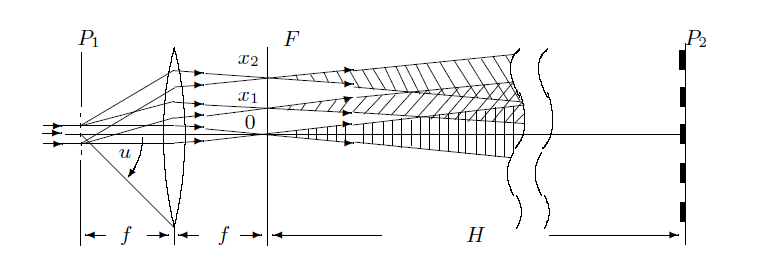
\includegraphics[width =  0.9\textwidth]{img}
		\caption{Образование изображения в объективе микроскопа. $P_1$ -- плоскость предмета, $F$ -- задняя фокальная плоскость объектива, $P_2$ -- плоскость, сопряжённая с предметной плоскостью. В плоскости $P_2$ световые пучки сильно перекрываются.}
		\label{img}
	\end{figure}

	Схема модели проекционного микроскопа приведена на рис. \ref{scheme}. Предметом служат сетки, расположенные в кассете. Смена сеток осуществляется поворотом внешнего кольца кассеты.
	
	\begin{figure}[H]
		\centering
		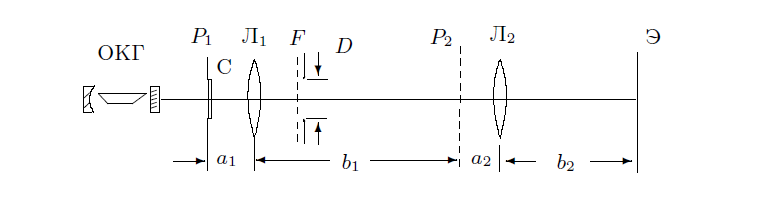
\includegraphics[width =  \textwidth]{scheme}
		\caption{Схема экспериментальной установки -- модель проекционного микроскопа.}
		\label{scheme}
	\end{figure}

	Излучение лазера (ОКГ) почти перпендикулярно падает на сетку С, установленную вблизи фокальной плоскости линзы $\text{\CYRL}_1$ -- объектива микроскопа. В нашей модели линза $\text{\CYRL}_1$ выбирается достаточно длиннофокусной ($f\approx 10$~ см), т.к. размер первичного изображения в фокальной плоскости $F$ должен быть не слишком малым, чтобы дополнительными диафрагмами можно было влиять на вторичное изображение в плоскости $P_2$. Вторичное изображение из плоскости $P_2$ проецируется на экран Э линзой $\text{\CYRL}_2$ (короткофокусной, чтобы изображение на экране было крупнее). Во избежание микротравм глаза от излучения лазера не следует использовать эту линзу традиционным образом как окуляр микроскопа.
	
	\newpage
	\section{Выполнение работы.}
	\subsection{Определение периода решёток по их пространственному спектру.}
	
	Определим расстояние между соседними дифракционными максимумами, измерив расстояние между удалёнными друг от друга максимумами (горизонтальными) и число промежутков между ними. Проведём измерение для пяти разных сеток. Результаты занесём в таблицу \ref{t1}.
	
	\begin{table}[H]
		\centering
		\caption{Измерение периода решёток (с помощью спектра).}
		\label{t1}
		\begin{tabular}{c|c|c} \toprule
			Решётка № & Расстояние, см & Число промежутков \\ \midrule
			$1$       & $14.3$         & $4$               \\
			$2$       & $14.4$         & $6$               \\
			$3$       & $14.3$         & $12$              \\
			$4$       & $7.1$          & $12$              \\
			$5$       & $8.1$          & $18$              \\ \bottomrule
		\end{tabular}
	\end{table}

	Измерим расстояние $H$ от сетки до экрана: $H = 134~\text{см}$.
	
	Запишем длину волны лазера, указанную на установке: $\lambda = 532~\text{нм}$.
	
	\subsection{Определение периода решёток по изображению, увеличенному с помощью модели микроскопа.}
	
	Соберём модель проекционного микроскопа (рис. \ref{scheme}).
	
	Определим расстояния $a_1, b_1, a_2, b_2$. Измерим периоды изображений сеток на экране. Данные занесём в таблицу \ref{t2}.
	

	\begin{table}[H]
		\centering
		\caption{Измерение периода решётки (с помощью микроскопа).}
		\label{t2}
		\begin{tabular}{c|c|c|c|c|c} \toprule
			Решётка № & Период изображения, мм & $b_2,~\text{см}$ & $a_2+b_1,~\text{см}$ & $a_1,~\text{см}$      & $a_2,~\text{см}$       \\ \midrule
			$1$         & $0.93$                 & $69$             & $44$                 & \multirow{5}{*}{$16$} & \multirow{5}{*}{$3.2$} \\
			$2$         & $1.4$                  & $69$             & $44$                 &                       &                        \\
			$3$         & $3$                    & $68.5$           & $44.5$               &                       &                        \\
			$4$         & $6$                    & $68.5$           & $44.5$               &                       &                        \\
			$5$         & $8$                    & $67$             & $46$                 &                       &                       \\ \bottomrule
		\end{tabular}
	\end{table}

	\subsection{Определение периодов решёток по оценке разрешающей способности микроскопа.}

	Поместим щелевую диафрагму с микрометрическим винтом в фокальную плоскость $F$ линзы $\text{\CYRL}_1$. Определим для каждой решётки минимальный размер диафрагмы $D$, при котором на экране ещё видно изображение сетки (при меньших размерах щели изображение выглядит как одномерная решётка). Занесём результаты в таблицу \ref{t3}.

	\begin{table}[H]
		\centering
		\caption{Измерение периода решёток (метод разрешающей способности).}
		\label{t3}
		\begin{tabular}{c|c|c|c|c|c} \toprule
			Решётка №       & $1$    & $2$    & $3$    & $4$    & $5$ \\ \midrule
			Размер щели, мм & -- & $3.37$ & $1.66$ & $1.05$ & $0.72$  \\ \bottomrule
		\end{tabular}
	\end{table}
	
	\subsection{Пространственная фильтрация и мультиплицирование.}
	
	Проделаем качественный опыт по пространственной фильтрации. Подберём сетку средних размеров с достаточно крупным вторичным изображением (метка "3"). Ширину щели подберём так, чтобы она свободно пропускала максимум нулевого порядка и не пропускала максимумы первого порядка, расположенные в поперечном направлении. Поворачивая щель относительно оси системы, получим изображение решёток при различных ориентациях щели: для вертикального и горизонтального положения, а также для наклонного положения под углом 45\degree, когда пропускаются максимумы с $m_x = m_y$.
	
	
	Для наблюдения явления мультиплицирования поменяем местами сетку С и щель D: сначала, не трогая линз, получим на экране резкое изображение щели, а затем в фокальной плоскости $F$ объектива поставим кассету с сетками, которые будут <<рассекать>> фурье-образ щели.
	
	Подберём такую ширину входной щели $D$, чтобы на экране можно было наблюдать мультиплицированное изображение для всех сеток.
	
	\section{Обработка результатов.}
	\begin{enumerate}
		\item По измерениям спектров (таблица \ref{t1}) определим дифракционные углы $\theta_x$ и рассчитаем периоды решёток по формуле \eqref{f1}.
	

	\begin{table}[H]
		\centering
		\caption{Периоды решёток (метод спектра).}
		
		\begin{tabular}{c|c|c} \toprule
			Решётка № & $\theta_x,~\text{рад}$ & $d,~\text{мкм}$ \\ \midrule
			$1$       & $0.053$                & \textbf{20}            \\
			$2$       & $0.054$                & \textbf{30}            \\
			$3$       & $0.053$                & \textbf{60}            \\
			$4$       & $0.026$                & \textbf{120}           \\
			$5$       & $0.030$                & \textbf{160}          \\ \bottomrule
		\end{tabular}
	\end{table}

	\item По измерениям увеличенных с помощью микроскопа изображений сеток 
	
	(таблица \ref{t2}) рассчитаем их периоды и сравним с результатами, полученными ранее.
	

	\begin{table}[H]
		\centering
		\caption{Периоды решёток (определение с помощью микроскопа).}
		\label{t4}
		\begin{tabular}{c|c|c} \toprule
			Решётка № & Увеличение            & $d,~\text{мкм}$ \\ \midrule
			$1$       & \multirow{5}{*}{$55$} & \textbf{17}   \\
			$2$       &                       & \textbf{25}   \\
			$3$       &                       & \textbf{54}   \\
			$4$       &                       & \textbf{109}  \\ 
			$5$       &                       & \textbf{143} \\ \bottomrule
		\end{tabular}
	\end{table}

	Результаты опытов практически совпадают.

	\item По измерениям со щелью (таблица \ref{t3}) рассчитаем по формуле \eqref{f2} минимальное расстояние (период решётки $d$), разрешаемое микроскопом, и сравним с результатами предыдущих измерений.
	
	\begin{table}[H]
		\centering
		\caption{Периоды решёток (оценка разрешающей способности микроскопа).}
		\label{t5}
		\begin{tabular}{c|c|c|c|c|c} \toprule
			Решётка №       & $1$ & $2$           & $3$         & $4$          &  $5$          \\ \midrule
			$d,~\text{мкм}$ & --  & \textbf{35} & \textbf{70} & \textbf{111} & \textbf{163} \\ \bottomrule
		\end{tabular}
	\end{table}

	Эти результаты также близки к полученным ранее.
	
	\item Для проверки теории Аббе построим график зависимости $d = f(1/D)$, взяв периоды сеток, определённые по спектру (рис \ref{itog}).
	
	\begin{figure}[H]
		\centering
		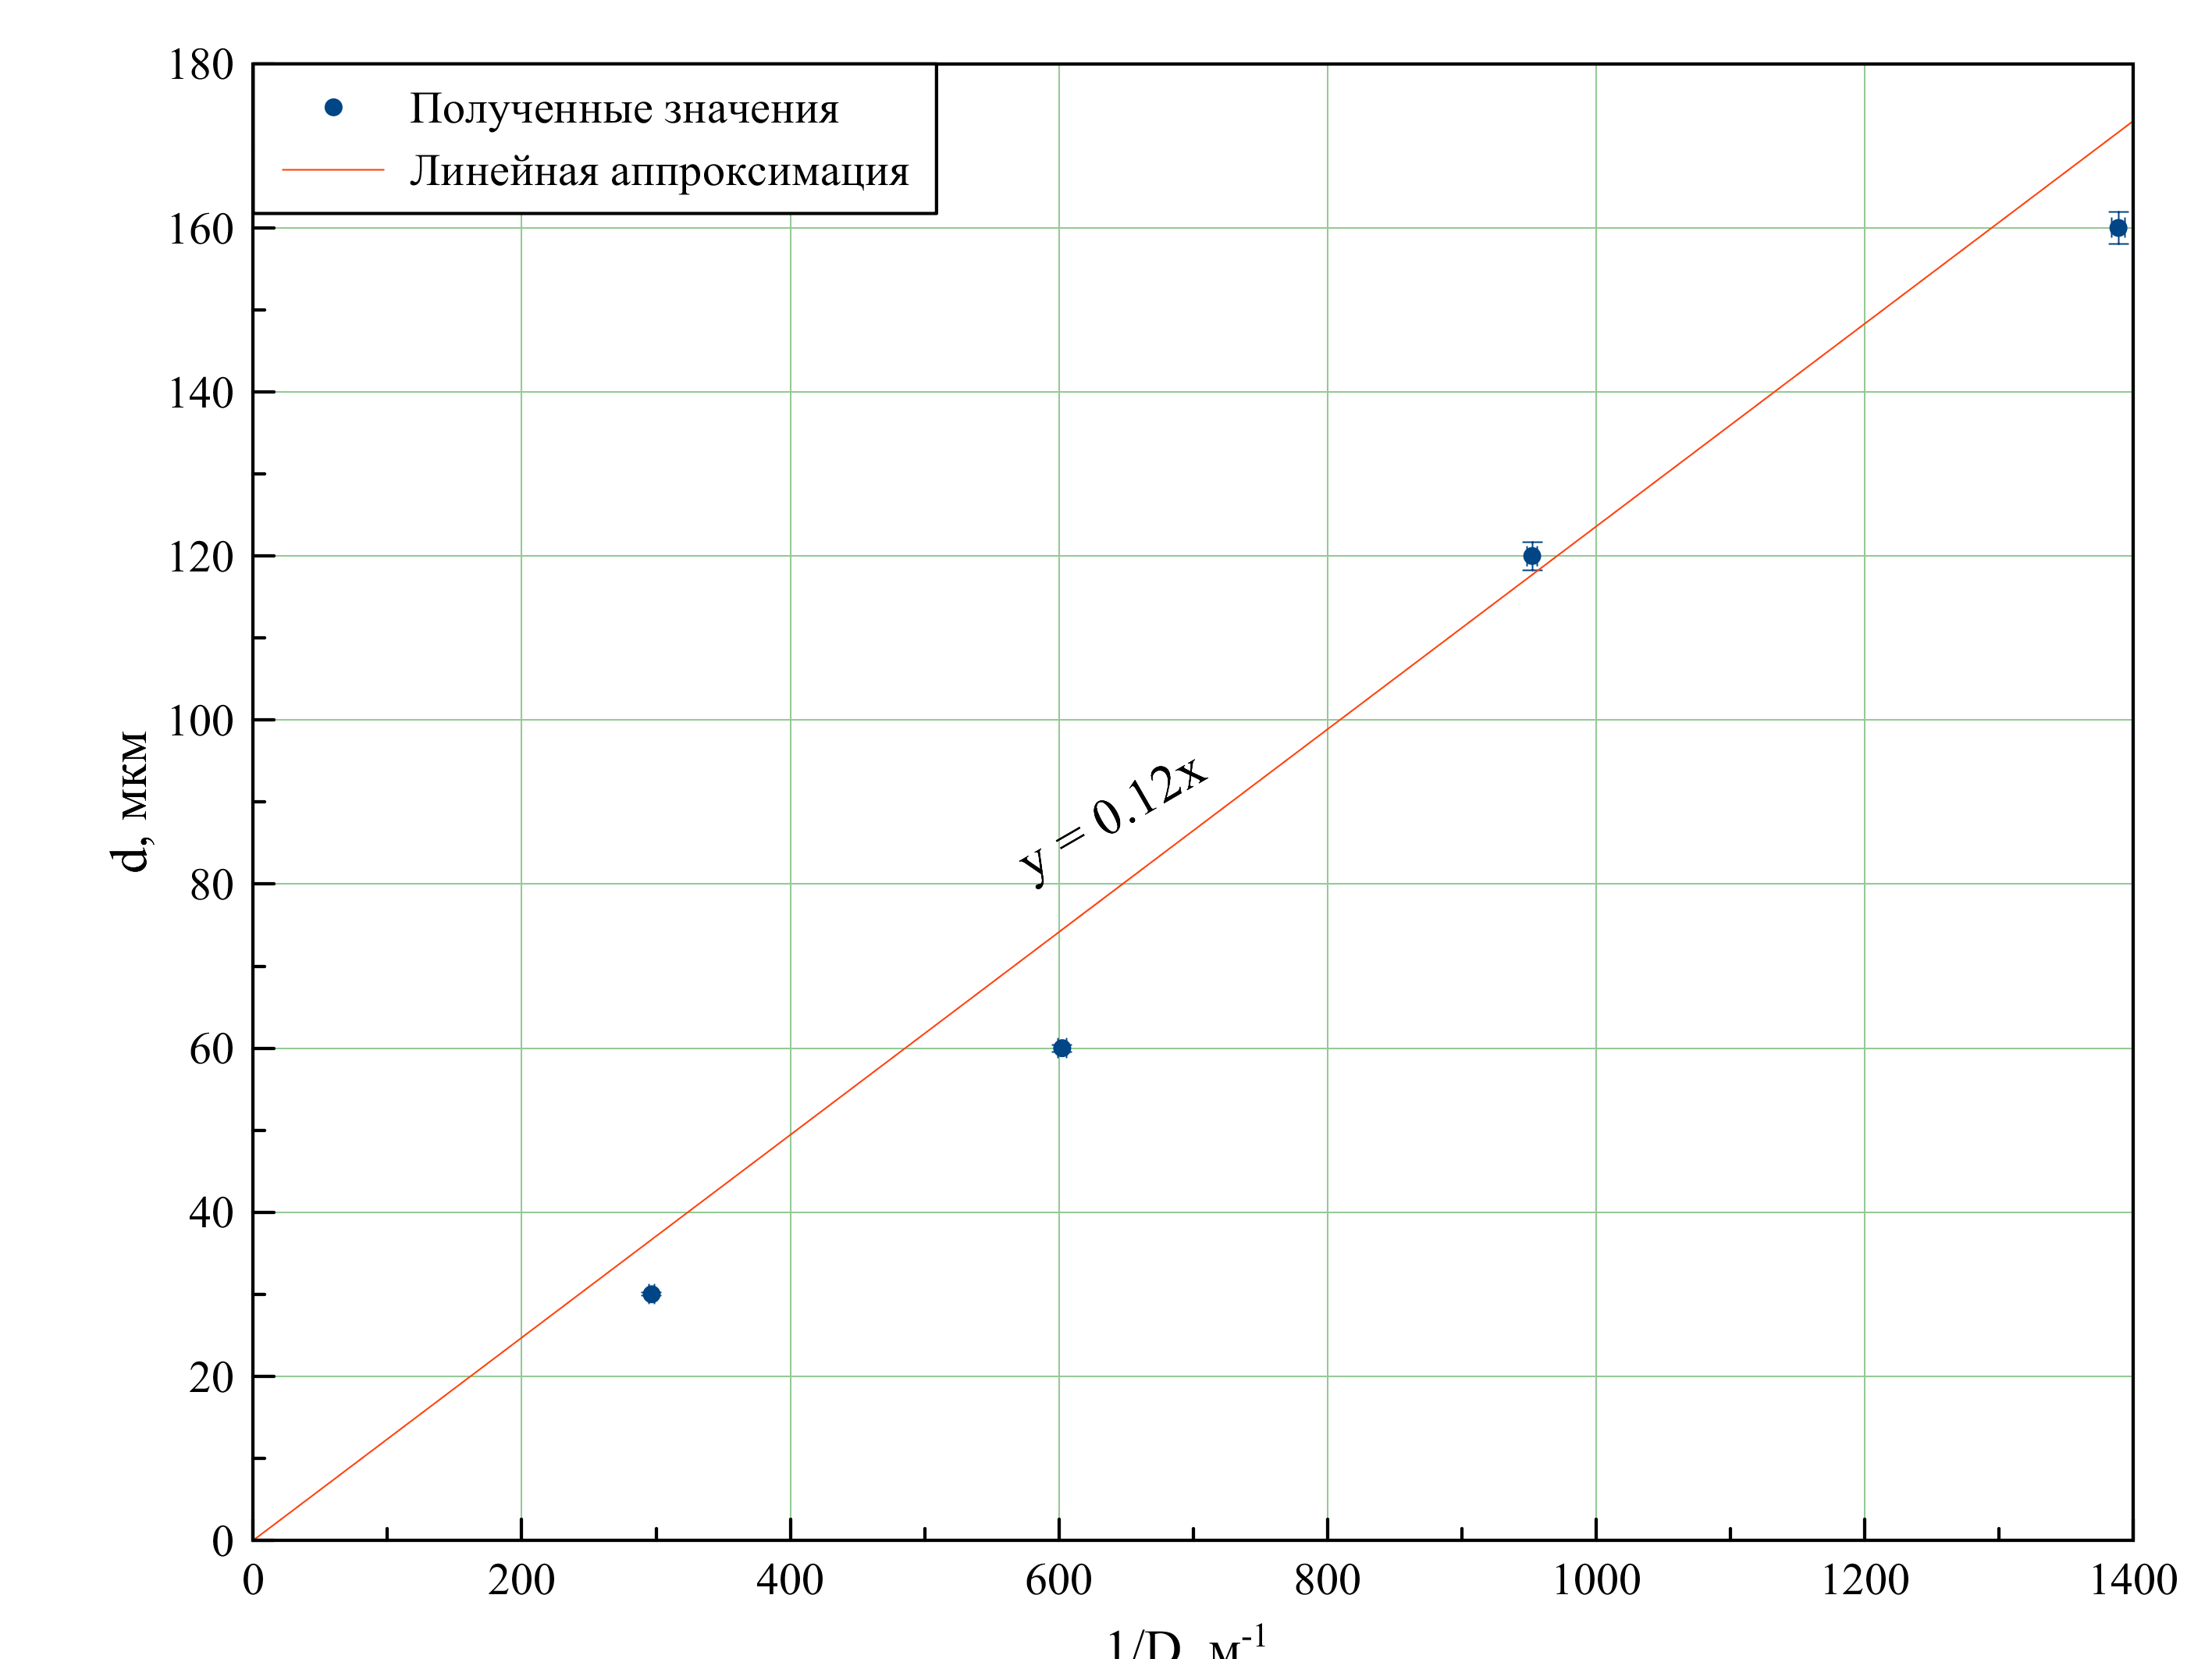
\includegraphics[width =  0.8\textwidth]{itog}
		\caption{Подтверждение теории Аббе.}
		\label{itog}
	\end{figure}

	Из графика видно, что зависимость близка к линейной $\Rightarrow$ теория Аббе выполняется.
	
	\item а) Отразим полученные изображения пространственной фильтрации на рис. \ref{ris1}
	
	\begin{figure}[H]
		\centering
		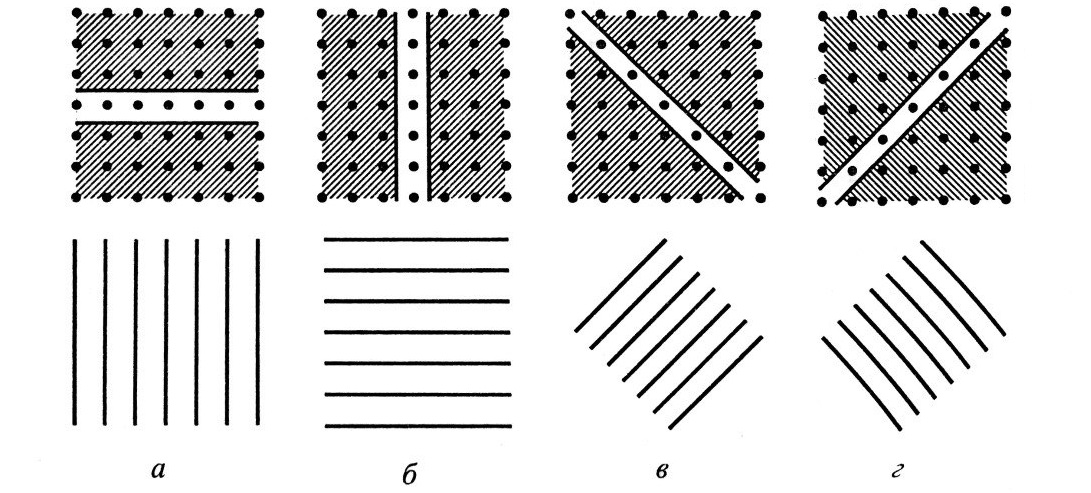
\includegraphics[width =  0.8\textwidth]{ris1}
		\caption{Пространственная фильтрация.}
		\label{ris1}
	\end{figure}

	
	
	 Ряд максимумов (рис. \ref{ris1}(а)) аналогичен дифракционной картине от одномерной решётки с вертикальными щелями. Поэтому оптическое изображение квадратной сетки при введении горизонтальной щели перейдёт в систему вертикальных полос. Аналогично для рис. \ref{ris1}(б).
	 
	 Если щель повернуть параллельно диагонали сетки (рис. \ref{ris1}(в и г)), то она   выделит прямолинейный ряд максимумов, параллельной той же диагонали, причём расстояния между максимумами увеличатся в $\sqrt{2}$ раз. В результате оптическое изображение сетки перейдёт в систему наклонных полос, перпендикулярных к щели, а сами полосы сделаются в $\sqrt{2}$ раз уже.	
	 
	 \textbf{Д.С. Рождественский указал, что непосредственной причиной появления ложных структур в этих опытах (опытах Аббе) является \textit{дифракция света на экранирующей сетке}.} 
	 
	 б) Явление мультиплицирования изображено на рис. \ref{multi}
	 
	 \begin{figure}[H]
	 	\centering
	 	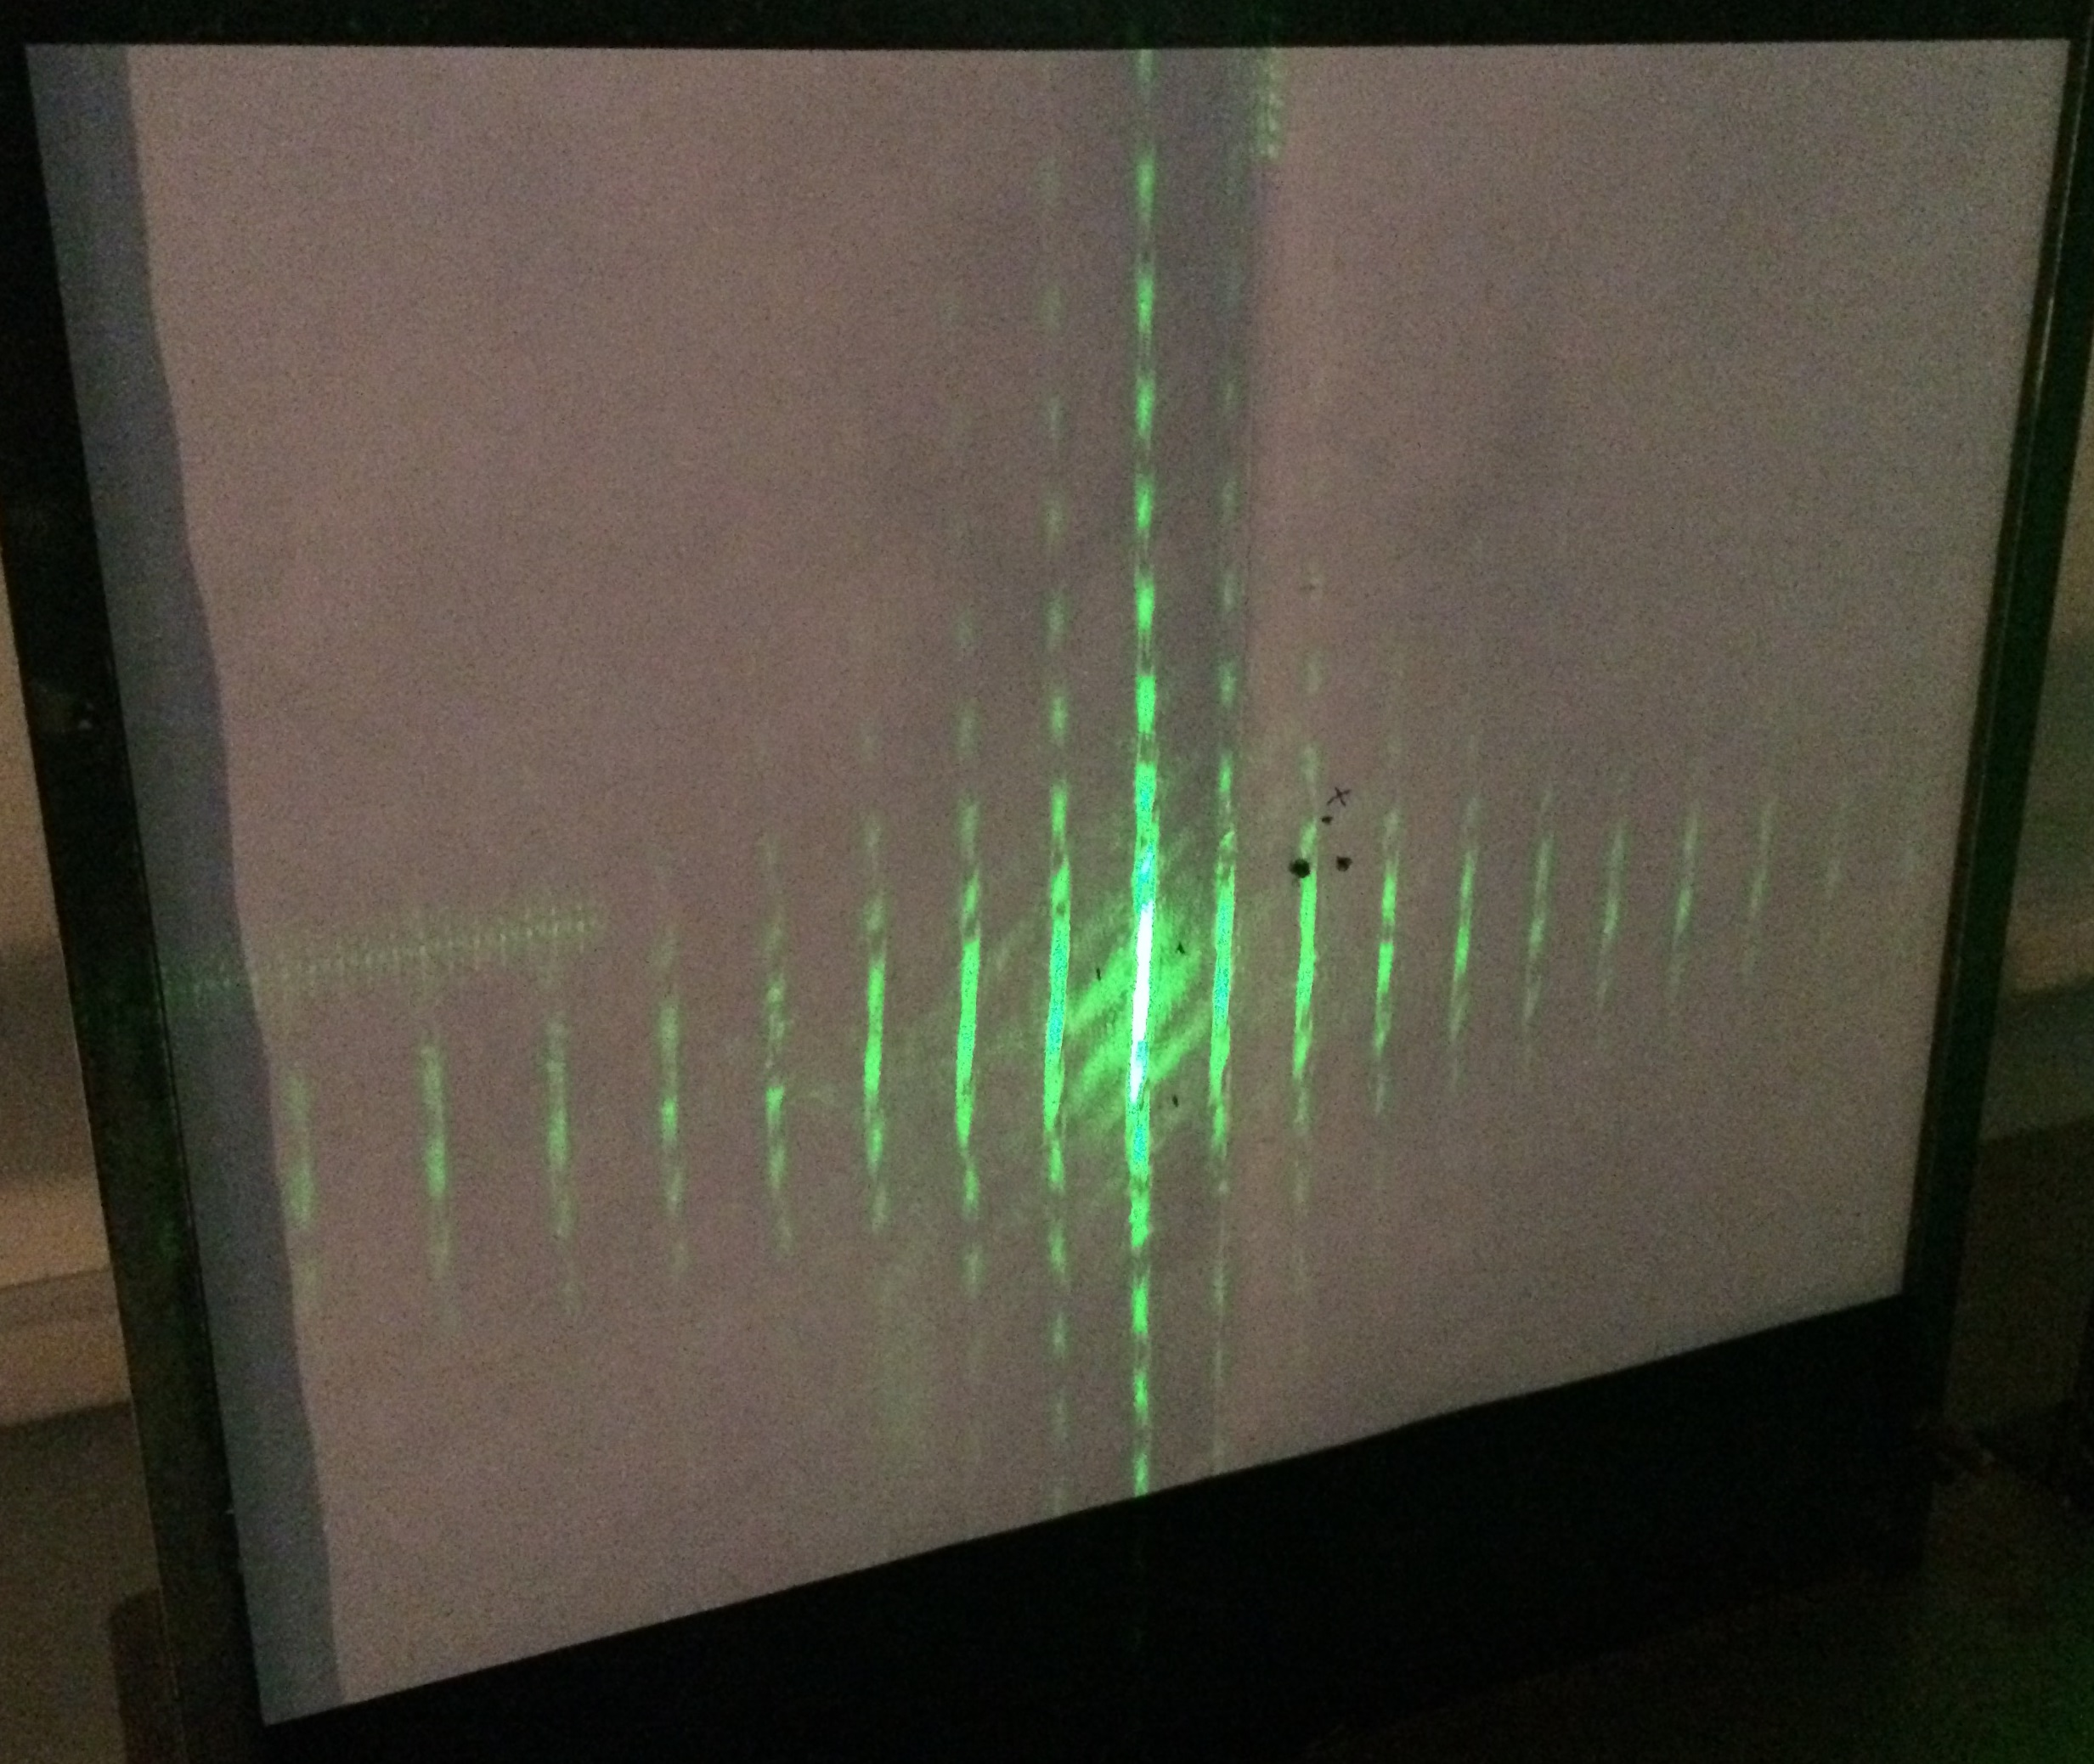
\includegraphics[width =  0.5\textwidth]{multi}
	 	\caption{Пространственная фильтрация.}
	 	\label{multi}
	 \end{figure}
 
 	Данное явление связано с тем, что фильтрующая решётка пропускает дискретный спектр компонент, что в свою очередь делает возможным представление изображения в плоскости $\text{\CYRP}_2$ в виде периодического.
 
 	Также было установлено, что при смене дифракционной сетки с меньшим периодом на сетку с большим периодом, период изображения уменьшается. Данный факт подтверждается формулами.
	
	\end{enumerate}

	\section{Вывод.}

	\begin{itemize}
		\item В ходе данной лабораторной работы был измерен период дифракционной решётки. Значения, полученные различными способами, оказались достаточно близкими.
		
		\item Был определён дифракционный предел разрешения объектива микроскопа методом Аббе, а также была проверена теория Аббе.
		
		\item Были изучены явления пространственной фильтрации и мультиплицирования.
	\end{itemize}
	

\end{document}